\documentclass[12pt]{article}
\usepackage{url,graphicx,tabularx,array,geometry,enumitem,amsmath}
\setlength{\parskip}{1ex} %--skip lines between paragraphs
\setlength{\parindent}{0pt} %--don't indent paragraphs

%-- Commands for header
\renewcommand{\title}[1]{\textbf{#1}\\}
\renewcommand{\line}{\begin{tabularx}{\textwidth}{X>{\raggedleft}X}\hline\\\end{tabularx}\\[-0.5cm]}
\newcommand{\leftright}[2]{\begin{tabularx}{\textwidth}{X>{\raggedleft}X}#1%
& #2\\\end{tabularx}\\[-0.5cm]}

%\linespread{2} %-- Uncomment for Double Space
\begin{document}

\title{Digital Signal Processing - Assignment 3}
\line
\leftright{\today}{Stephanie Lund (2555914)\\Aljoscha Dietrich(2557976)} %-- left and right positions in the header

\section*{Exercise 1}
By solving the two constraints $\lvert H_c(j 0.2\pi) \rvert \geq 0.89125$ and $\lvert H_c(j 0.3\pi) \rvert \leq 0.17783$, we get:
\begin{align*}
	N &= 6\\
	\omega_c &= 0.70474
\end{align*}

The graph of the magnitude of the frequency response $\lvert H_c(j\omega) \rvert$ is then:

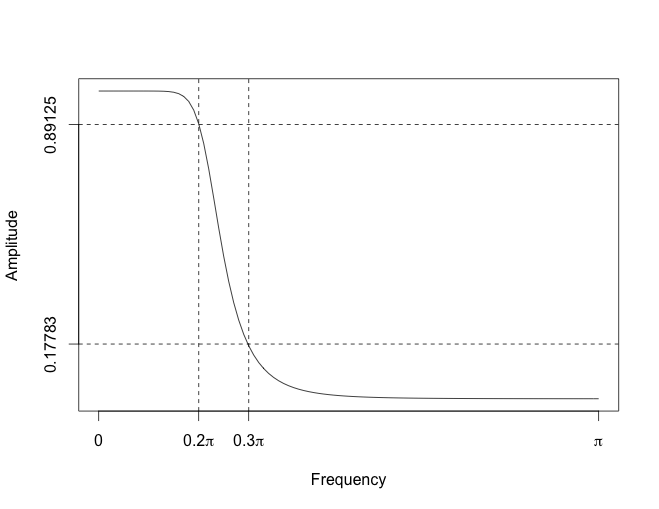
\includegraphics[scale=0.65]{hw3-1.png}

\section*{Exercise 2}

\subsection*{2.1}
\begin{enumerate}[label=\alph*)]
\item The minimum sampling frequency is 10kHz, so $T = \frac{1}{f_s} \geq \frac{1}{10,000}$.

\item $2\pi f = \frac{\pi/8}{T}$. Solve for $f$ to get $625 kHz$.

\item Solve the above equation using $T = \frac{1}{20,000}$ to get $f = 1250 kHz$.


\end{enumerate}

\subsection*{2.2}
In all cases, upsampling by 3 and then downsampling by 3 doesn't change the signal. After applying the low-pass filter to cut off all frequencies above $\frac{\pi}{3}$, $(a)$ and $(c)$ remain unchanged, as their frequencies are below the cutoff, but $(b)$ will be changed, since the frequency is above the cutoff.

\section*{Exercise 3}
The code is located in the file hw3.m. The settings chosen for the low-pass filter were a Butterworth filter with $N = 10$ and $\omega_c = 0.02$ radians.

\section*{Bonus}
$T_1$ and $T_2$ are equivalent if $N$ and $M$ are relatively prime, or if $N = M$.


\end{document}
